\section{EnergyScope Pathway: The right model} 
\label{app:ESPathway_choice}

``\textit{Only when single-model results are contextualized by the model's position in the larger ensemble, the reader would be able to have a complete and correct interpretation of the output}" \cite{dekker2023identifying}. Energy system models of varying complexity are valuable tools for guiding policymakers and projecting future trends. These models enable the exploration of different energy scenarios and the assessment of their consequences. Specifically, techno-economic models play a crucial role in identifying technically feasible pathways for the energy transition while considering the associated economic costs. These models can be classified based on two key factors: technical resolution and simulation horizon, as illustrated in Figure \ref{fig:energy_models_classification}.


\begin{figure}[!htbp]
\centering
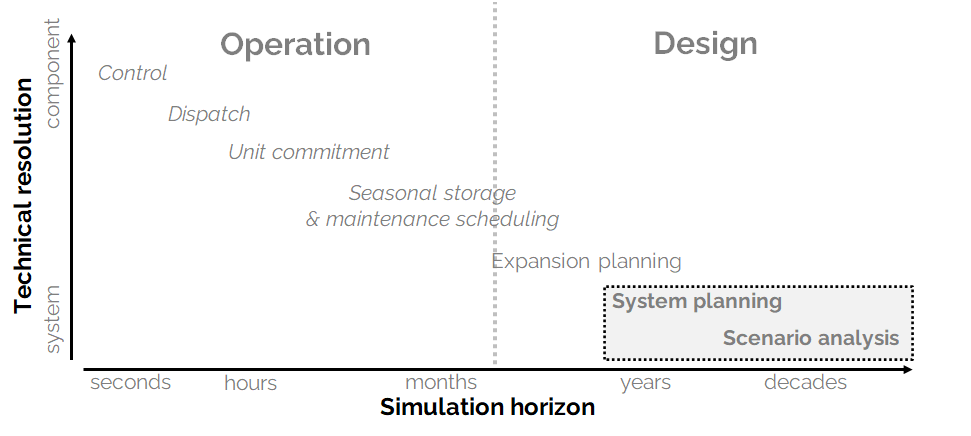
\includegraphics[width=\textwidth]{Models_classification.png}
\caption{Model can be classified by their core focus: \textbf{Operation} or \textbf{Design}. These categories can be broken down into subcategories. This work focuses on the system planning and scenario analysis models. Inspired from \cite{palmintier2013incorporating}. }
\label{fig:energy_models_classification}
\end{figure}


Increasing the technical resolution of energy system models often comes at the expense of a shorter simulation horizon, and vice versa. For instance, day-ahead grid operation models prioritise accurate grid resolution and capacity reserves in case of foreseeable deviations, but they may not incorporate long-term market trends. Different model classes cater to various needs, with decreasing technical resolution. These include machine-level control, network dispatch, unit commitment, maintenance, power plant expansion, planning for new infrastructure, and scenario analysis. Each class serves a specific purpose, from fine-grained control within a machine to the exploration of multiple assumptions across different scenarios.

% Specific need & criteria

In accordance with the previous classification, models aimed at aiding decision-makers in the energy transition primarily fall under the categories of planning and scenario analysis, with a lower technical resolution than the other classes of model (see Figure \ref{fig:energy_models_classification}). Nonetheless, ensuring technical accuracy is of paramount importance to ensure the effective performance of future energy systems. Hence, these models should meet the following requirements as a minimum:
(i) assessment of intermittent renewable energy integration thanks to an \textbf{hourly resolution} spanning a one-year time horizon;
(ii) accounting for the \textbf{whole-energy system} by including all energy (\ie heat, electricity and mobility) and non-energy flows in different sectors, accounting for their respective greenhouse gas emissions, as well as all resources, conversion processes, and storage technologies;
(iii) exploration of all available options through the \textbf{optimisation of investments and operations};
(iv) consideration of long-term investments throughout the \textbf{transition pathway} process (\ie 30 years up to 2050, in our case); and
(v) ensuring a reasonable \textbf{computational time} (\ie less than one hour on a personal laptop) for analysing different trajectories.
Additionally, to enhance result reproducibility and user understanding, it is advantageous for such models to:
(vi) maintain transparency and preferably be \textbf{open-source}, with accessible data and accompanied by collaborative documentation.

%These requirements can be transposed into criteria that a model should match:
%(i) it should have an hourly resolution spanning a one-year time horizon;
%(ii) it should encompass the entire energy system, including all types of demands (such as heat, electricity, mobility, and non-energy)
%%\footnote{Non-energy demand is often omitted in models while it represents up to 10\%  of worldwide energy demand and up to 20\% in some countries \cite{rixhon2022integration}. \citet{eurostat2019energy} defines the non-energy demand as `\emph{energy products used as raw materials in different sectors, not consumed as a fuel or transformed into another fuel}´.}
%, as well as all resources, conversion processes, and storage technologies;
%(iii) it should optimise the system design, accounting for all the options;
%(iv) it should have a long-term investment horizon, spanning several decades;
%(v) its computational time should be reasonable, typically less than one hour on a personal laptop;
%(vi) it should be open-source, with accessible data and comprehensive documentation.

These requirements are commonly found in reviews on energy system models. In 2010, \citet{Connolly2010} reviewed 68 tools, considering similar criteria (\ie (i-iv) and (vi)), along with others such as the ``popularity'' of the models via the number of downloads/sales or the integration of economic market equilibrium. Eight years later, \citet{lopion2018review} enriched the review of \citet{Connolly2010} using similar critieria and including models developed in the 2010s. In 2014, \citet{pfenninger2014energy} pointed out the current paradigms and challenges to face as well as the emerging approaches to address them in the 21st century energy systems modeling community.  Besides the behavioral and social factors, they also highlighted the challenges related to mutli-sectorial systems, time and space resolution or the open-accessibility of data and models and their ability to account for uncertainties. In 2019, \citet{prina2019transition} reviewed 12 ``\emph{most established}" models, focusing on criteria (i-ii) and (iv). This review was followed by a classification where criteria (i-iv) were taken into account \cite{prina2020classification}. In 2021, \citet{chang2021trends} conducted a survey-based review of 42 models for energy transition modelling, covering all criteria except computational time.
Based on these reviews, models are compared based on all the previous criteria except the computational time (v) (see Table \ref{tab:intro_soa}). Indeed, the latter is hard to compare as models are not applied to the same case study and the information is rarely given. The table includes only the models that achieved partially at least four out of the five criteria. We endeavored to update the model's information by consulting the model's website and repository, yet there is a possibility that some information might have been overlooked or omitted inadvertently.

\begin{table}[!htbp]
\caption{Comparison of existing models that partially satisfy at least four of the five criteria (in alphabetical order). Legend: \checkmark criterion satisfied; {\color{lightgray} \checkmark} criterion partially satisfied; {\color{gray} \xmark} criterion not satisfied. Data from \cite{Connolly2010,prina2020classification,chang2021trends,prina2019transition}}
\label{tab:intro_soa}
\begin{minipage}{\textwidth}
\centering
\resizebox{\textwidth}{!}{
\begin{tabular}{lcccccc}
\toprule
\textbf{Model} & \textbf{Ref.} & \textbf{Hourly} & \textbf{\parbox{2cm}{\centering Whole-energy}}& \textbf{\parbox{2cm}{\centering Optimis. invest. \& operation}} & \textbf{Pathway} & \textbf{\parbox{2cm}{\centering Open-source}} \\
\midrule
Calliope & \cite{Atlason2014,Calliope} & \checkmark & \checkmark & \checkmark & {\color{gray} \xmark}\footnote{Topic is being discussed in the chat of their repository but not yet included in their documentation.} & \checkmark \\
COMPOSE & \cite{COMPOSE} & \checkmark & \checkmark & \checkmark & \checkmark & {\color{lightgray} \checkmark}\footnote{\label{foot:freeundersomespecial}`\emph{Free under some special conditions}´.} \\
DER-CAM & \cite{popovic2017mixed,dercam_website} & \checkmark & {\color{lightgray} \checkmark}\footnote{\label{foot:transportnotsaid} Transport not accounted for.}\footnote{\label{foot:industrynotaccounted} Industry not accounted for.} & \checkmark & {\color{gray} \xmark} \footnote{\label{foot:notpathway} Not specified but time horizon is 1 year.} & {\color{lightgray} \checkmark} \footnote{\label{foot:freeware} Freeware.} \\
DIETER & \cite{zerrahn2017long} & \checkmark & {\color{lightgray} \checkmark} \footref{foot:industrynotaccounted}\footnote{\label{foot:dhnnotaccounted} \gls{DHN} not accounted for.} & \checkmark & {\color{gray} \xmark}\footref{foot:notpathway} & \checkmark \\
E2M2 & \cite{E2M2} & \checkmark & {\color{lightgray} \checkmark} \footref{foot:transportnotsaid}\footref{foot:industrynotaccounted}\footnote{\label{foot:decLTHnotaccounted} Individual heating not accounted for.} & \checkmark & \checkmark & {\color{gray} \xmark}\footnote{\label{foot:paidlicenced} Commercially (paid) licensed.} \\
EMPIRE & \cite{backe2022empire} & \checkmark & {\color{gray} \xmark} \footref{foot:transportnotsaid}\footref{foot:industrynotaccounted}\footref{foot:dhnnotaccounted}\footref{foot:decLTHnotaccounted} & \checkmark & \checkmark & {\color{lightgray} \checkmark}\footref{foot:freeundersomespecial} \\
Ener. Trans. Model & \cite{ETM} & \checkmark & \checkmark & {\color{gray} \xmark} \footnote{The ETM is a simulation model with a simple merit order 'optimisation' for electricity, flexibility and heat.} & \checkmark & \checkmark \\
EnergyPLAN & \cite{lundenergyplan} & \checkmark & \checkmark & {\color{gray} \xmark} \footnote{\label{foot:simulation} Simulation model.} & {\color{gray} \xmark} \footnote{\label{foot:notpathwaystated} Yearly horizon without pathway.} & {\color{lightgray} \checkmark}\footref{foot:freeware} \\
energyRt & \cite{EnergyRT} & \checkmark & \checkmark & {\color{lightgray} \checkmark} \footnote{\label{foot:invopt} EnergyRT optimises investments only.} & \checkmark & \checkmark \\
EnergyScope TD & \cite{limpens2019energyscope} & \checkmark & \checkmark & \checkmark & {\color{gray} \xmark} \footref{foot:notpathwaystated} & \checkmark \\
Enertile & \cite{enertile} & \checkmark & \checkmark \footref{foot:industrynotaccounted} & \checkmark & \checkmark & {\color{gray} \xmark} \footnote{Only for internal use.} \\
ESO-XEL & \cite{heuberger2017electricity} & \checkmark & {\color{gray} \xmark}\footref{foot:transportnotsaid}\footref{foot:industrynotaccounted}\footref{foot:dhnnotaccounted}\footref{foot:decLTHnotaccounted} & \checkmark & \checkmark & \checkmark \\
GENeSYS-MOD & \cite{loffler2017designing} & \checkmark & \checkmark & \checkmark &  \checkmark
%\footnote{\citet{loffler2017designing} applied a pathway transition, but the time resolution was increased to 12h and it uses 3 typical days over a year. \citet{bartholdsen2019pathways} performed a multi-regional pathway (16 nodes) for the case of Germany from 2020 to 2050 with a time step of 5 years. However, the time resolution is 16 time slices representing 4 hours per day and one day per season.}
 & \checkmark \\
H2RES & \cite{herc2021energy} & \checkmark & {\color{gray} \xmark}
%\footnote{\label{foot:h2res} In their review in 2021, \citet{prina2021bottom} classified H2RES as a simulation model on power sector only. In their work, \citet{herc2021energy} presented a new version of H2RES claiming to optimise the power system and partially represent other sectors. Their study applied the model to a transition pathway for Croatia. In the conclusion, it is claimed `\textit{H2RES offers practically unlimited potential for functionality expansion since it is an open-source program}´ which open the doors for future developments to encompass new features.}
&  {\color{lightgray} \checkmark}\footref{foot:h2res} & \checkmark & \checkmark \\ 
iHOGA & \cite{ihoga} & \checkmark & {\color{gray} \xmark}\footref{foot:transportnotsaid}\footref{foot:industrynotaccounted}\footref{foot:dhnnotaccounted}\footref{foot:decLTHnotaccounted} & {\color{lightgray} \checkmark} \footref{foot:invopt} & \checkmark & {\color{lightgray} \checkmark} \footref{foot:freeundersomespecial} \\
IMAKUS & \cite{kuhn2012iteratives} & \checkmark & {\color{lightgray} \checkmark}\footref{foot:transportnotsaid}\footref{foot:industrynotaccounted} & \checkmark & \checkmark & {\color{gray} \xmark} \footref{foot:paidlicenced} \\
OpenDSS & \cite{opendss} & \checkmark & \checkmark & {\color{gray} \xmark} \footref{foot:simulation} & \checkmark & \checkmark \\
Plexos & \cite{energyexemplarplexos9} & \checkmark & {\color{lightgray} \checkmark}\footnote{Does not account for all sectors but allow to implement them according to \citet{waucquez2023validation}.} & \checkmark & \checkmark & {\color{gray} \xmark}\footref{foot:paidlicenced}  \\
PyPSA & \cite{brown2017pypsa,PyPsa} & \checkmark & \checkmark & \checkmark & {\color{lightgray} \checkmark} \footnote{\citet{pedersen2022long} applied PyPSA to a whole energy system split in 37 nodes. Using a myopic approach, the model optimises the energy transition with a 3-hours resolution). } & \checkmark \\
RamsesR & \cite{energistyrelsen2023ramses} & \checkmark & {\color{lightgray} \checkmark}\footref{foot:transportnotsaid}\footref{foot:industrynotaccounted}\footref{foot:decLTHnotaccounted} & \checkmark  & \checkmark & \checkmark \\
ReEDS & \cite{short2011regional} & {\color{gray} \xmark}\footnote{ Seasonal time slice.} & {\color{lightgray} \checkmark}\footref{foot:industrynotaccounted}\footref{foot:dhnnotaccounted}\footref{foot:decLTHnotaccounted} & \checkmark & \checkmark & {\color{lightgray} \checkmark} \footref{foot:freeundersomespecial} \\
TIMES & \cite{loulou2005documentation} & \checkmark & \checkmark & \checkmark & \checkmark & \checkmark\footnote{Model is now open-source with limited access to data \cite{openmod_times_description}.} \\
\bottomrule
\end{tabular}}
\end{minipage}
\end{table}


%\begin{table}[!htbp]
%\caption{Comparison of existing models that partially satisfy at least four of the five criteria (in alphabetical order). Legend: \checkmark criterion satisfied; {\color{lightgray} \checkmark} criterion partially satisfied; {\color{gray} \xmark} criterion not satisfied. Data from \cite{Connolly2010,prina2020classification,chang2021trends,prina2019transition} (part B)}
%\label{tab:intro_soa_bis}
%\begin{minipage}{\textwidth}
%\centering
%\resizebox{\textwidth}{!}{
%\begin{tabular}{lcccccc}
%\toprule
%\textbf{Model} & \textbf{Ref.} & \textbf{Hourly} & \textbf{\parbox{2cm}{\centering Whole-energy}}& \textbf{\parbox{2cm}{\centering Optimis. invest. \& operation}} & \textbf{Pathway} & \textbf{\parbox{2cm}{\centering Open-source}} \\
%\midrule
%Calliope & \cite{Atlason2014,Calliope} & \checkmark & \checkmark & \checkmark & {\color{gray} \xmark}\footnote{Topic is being discussed in the chat of their repository but not yet included in their documentation.} & \checkmark \\
%COMPOSE & \cite{COMPOSE} & \checkmark & \checkmark & \checkmark & \checkmark & {\color{lightgray} \checkmark}\footnote{\label{foot:freeundersomespecial}`\emph{Free under some special conditions}´.} \\
%DER-CAM & \cite{popovic2017mixed,dercam_website} & \checkmark & {\color{lightgray} \checkmark}\footnote{\label{foot:transportnotsaid} Transport not accounted.}\footnote{\label{foot:industrynotaccounted} Industry not accounted} & \checkmark & {\color{gray} \xmark} \footnote{\label{foot:notpathway} Not specified but time horizon is 1 year.} & {\color{lightgray} \checkmark} \footnote{\label{foot:freeware} Freeware.} \\
%DIETER & \cite{zerrahn2017long} & \checkmark & {\color{lightgray} \checkmark} \footref{foot:industrynotaccounted}\footnote{\label{foot:dhnnotaccounted} \gls{DHN} not accounted.} & \checkmark & {\color{gray} \xmark}\footref{foot:notpathway} & \checkmark \\
%E2M2 & \cite{E2M2} & \checkmark & {\color{lightgray} \checkmark} \footref{foot:transportnotsaid}\footref{foot:industrynotaccounted}\footnote{\label{foot:decLTHnotaccounted} individual heating not accounted.} & \checkmark & \checkmark & {\color{gray} \xmark}\footnote{\label{foot:paidlicenced} Commercially (paid) licensed.} \\
%EMPIRE & \cite{backe2022empire} & \checkmark & {\color{gray} \xmark} \footref{foot:transportnotsaid}\footref{foot:industrynotaccounted}\footref{foot:dhnnotaccounted}\footref{foot:decLTHnotaccounted} & \checkmark & \checkmark & {\color{lightgray} \checkmark}\footref{foot:freeundersomespecial} \\
%Ener. Trans. Model & \cite{ETM} & \checkmark & \checkmark & {\color{gray} \xmark} \footnote{The ETM is a simulation model with a simple merit order 'optimisation' for electricity, flex and heat.} & \checkmark & \checkmark \\
%EnergyPLAN & \cite{lundenergyplan} & \checkmark & \checkmark & {\color{gray} \xmark} \footnote{\label{foot:simulation} Simulation model.} & {\color{gray} \xmark} \footnote{\label{foot:notpathwaystated} Yearly horizon without pathway.} & {\color{lightgray} \checkmark}\footref{foot:freeware} \\
%energyRt & \cite{EnergyRT} & \checkmark & \checkmark & {\color{lightgray} \checkmark} \footnote{\label{foot:invopt} EnergyRT optimises investments only, while iHOGA conducts optimisation and simulation without specifying timing or scope.} & \checkmark & \checkmark \\
%EnergyScope TD & \cite{limpens2019energyscope} & \checkmark & \checkmark & \checkmark & {\color{gray} \xmark} \footref{foot:notpathwaystated} & \checkmark \\
%Enertile & \cite{enertile} & \checkmark & \checkmark \footref{foot:industrynotaccounted} & \checkmark & \checkmark & {\color{gray} \xmark} \footnote{ Only for internal use.} \\
%ESO-XEL & \cite{heuberger2017electricity} & \checkmark & {\color{gray} \xmark}\footnote{\label{foot:transportnotsaid_bis} Transport not accounted.}\footnote{\label{foot:industrynotaccounted_bis} Industry not accounted}\footnote{\label{foot:dhnnotaccounted_bis} \gls{DHN} not accounted.}\footnote{\label{foot:decLTHnotaccounted_bis} individual heating not accounted.} & \checkmark & \checkmark & \checkmark \\
%GENeSYS-MOD & \cite{loffler2017designing} & \checkmark & \checkmark & \checkmark &  \checkmark\footnote{\citet{loffler2017designing} applied a pathway transition, but the time resolution was increased to 12h and it uses 3 typical days over a year. \citet{bartholdsen2019pathways} performed a multi-regional pathway (16 nodes) for the case of Germany from 2020 to 2050 with a time step of 5 years. However, the time resolution is 16 time slices representing 4 hours per day and one day per season.} & \checkmark \\
%H2RES & \cite{herc2021energy} & \checkmark & {\color{gray} \xmark}\footnote{\label{foot:h2res} In their review in 2021, \citet{prina2021bottom} classified H2RES as a simulation model on power sector only. In their work, \citet{herc2021energy} presented a new version of H2RES claiming to optimise the power system and partially represent other sectors. Their study applied the model to a transition pathway for Croatia. In the conclusion, it is claimed `\textit{H2RES offers practically unlimited potential for functionality expansion since it is an open-source program}´ which open the doors for future developments to encompass new features.} &  {\color{lightgray} \checkmark}\footref{foot:h2res} & \checkmark & \checkmark \\ 
%iHOGA & \cite{ihoga} & \checkmark & {\color{gray} \xmark}\footref{foot:transportnotsaid_bis}\footref{foot:industrynotaccounted_bis}\footref{foot:dhnnotaccounted_bis}\footref{foot:decLTHnotaccounted_bis} & {\color{lightgray} \checkmark} \footnote{\label{foot:invopt_bis} iHOGA conducts optimisation and simulation without specifying timing or scope.} & \checkmark & {\color{lightgray} \checkmark} \footnote{\label{foot:freeundersomespecial_bis}`\emph{Free under some special conditions}´.} \\
%IMAKUS & \cite{kuhn2012iteratives} & \checkmark & {\color{lightgray} \checkmark}\footref{foot:transportnotsaid_bis}\footref{foot:industrynotaccounted_bis} & \checkmark & \checkmark & {\color{gray} \xmark}\footnote{\label{foot:paidlicenced_bis} Commercially (paid) licensed.} \\
%OpenDSS & \cite{opendss} & \checkmark & \checkmark & {\color{gray} \xmark} \footnote{\label{foot:simulation_bis} Simulation model.} & \checkmark & \checkmark \\
%Plexos & \cite{energyexemplarplexos9} & \checkmark & {\color{lightgray} \checkmark}\footnote{Does not account for all sectors but allow to implement them according to \citet{waucquez2023validation}.} & \checkmark & \checkmark & {\color{gray} \xmark}\footref{foot:paidlicenced_bis}  \\
%PyPSA & \cite{brown2017pypsa,PyPsa} & \checkmark & \checkmark & \checkmark & {\color{lightgray} \checkmark} \footnote{\citet{pedersen2022long} applied PyPSA to a whole energy system split in 37 nodes. Using a myopic approach, the model optimises the energy transition with a 3-hours resolution). } & \checkmark \\
%RamsesR & \cite{energistyrelsen2023ramses} & \checkmark & {\color{lightgray} \checkmark}\footref{foot:transportnotsaid_bis}\footref{foot:industrynotaccounted_bis}\footref{foot:decLTHnotaccounted_bis} & \checkmark  & \checkmark & \checkmark \\
%ReEDS & \cite{short2011regional} & {\color{gray} \xmark}\footnote{ Seasonal time slice.} & {\color{lightgray} \checkmark}\footref{foot:industrynotaccounted_bis}\footref{foot:dhnnotaccounted_bis}\footref{foot:decLTHnotaccounted_bis} & \checkmark & \checkmark & {\color{lightgray} \checkmark} \footref{foot:freeundersomespecial_bis} \\
%TIMES & \cite{loulou2005documentation} & \checkmark & \checkmark & \checkmark & \checkmark & \checkmark\footnote{Model is now open-source with limited access to data \cite{openmod_times_description}.} \\
%\bottomrule
%\end{tabular}}
%\end{minipage}
%\end{table}


From Table \ref{tab:intro_soa}, four models almost check all the boxes (partially the pathway one): Calliope, GENeSYS-MOD, PyPSA and TIMES. \\

\myparagraph{Calliope}\\

\noindent
Calliope is a ``\emph{tool that makes it easy to build energy system models}'' at different geographical scale. Even if the framework offers the possibility of modelling multi-year systems, we did not find a relevant publication on this topic. In fact, the model is typically employed for snapshot analysis, \ie optimization of a target future year. Previous studies have used the model to investigate the phasing out of fossil and nuclear energies in a multi-regional UK power system \cite{pfenninger2015renewables}. More recently, the model has been applied to analyse a scenario of a multi-energy district in Switzerland \cite{pickering2021quantifying}. Moreover, the model has been used with decades of weather data. However, its application has been limited to assessing the impact of inter-year variability in wind and PV on the results, 
rather than evaluating a transition pathway \cite{pfenninger2017dealing}. \\

\myparagraph{GENeSYS-MOD}\\

\noindent
Similarly GENeSYS-MOD presents some limitations. This model is an application of the open-source energy modelling system (OSeMOSYS), itself represented as a model with a poor time discretisation and a heavy computational burden according to \cite{prina2019transition}. \citet{loffler2017designing} applied the model to the world by splitting it into 10 regions and most of the energy demand sectors, leaving to the user the choice of the time resolution.  For their application they used representative years with three days and two time slice per day. \\
%\cite{bartholdsen2019pathways} performed a similar study for the case of Germany with 16 time slices per representative years and motivated this choice as sufficient as \cite{welsch2014incorporating} demonstrates that it gives consistent results compared to using hourly time resolution over a year.  However, with limited number of time slices, storage technologies, especially the ones for inter-month storage, cannot be optimised and thus simplifies the non-yet solved challenge of intermittent renewable energy integration. 
%PyPSA, one of the most promising model thanks to its strong and active community, has also been used to perform a myopic transition \cite{pedersen2022long}.  

\myparagraph{PyPSA}\\

\noindent
Among the open-source models with an active community, PyPSA is one of the best-performing, with a large and active community, development at the state of the art, worldwide applications, and usage not only limited to academia. A study conducted by \citet{bartholdsen2019pathways} centered on Germany employed a representation comprising 16 time slices per representative year. This choice was substantiated by the work of \citet{welsch2014incorporating}, which demonstrated that this level of temporal granularity yields consistent results in comparison to hourly time resolution over a year. However, it is noteworthy that the utilization of a limited number of time slices may oversimplify the optimization of storage technologies, especially those designed for inter-month energy storage. This simplification can be viewed as a pragmatic approach to reduce the computational burden while over-simplifying the challenge of accurately integrating intermittent renewable energy sources. Furthermore, PyPSA, a modeling framework recognized for its robustness and active user community, has also been employed to investigate scenarios related to myopic transitions \cite{pedersen2022long}. \\

\myparagraph{TIMES}\\

\noindent
The TIMES model, short for The Integrated MARKAL-EFOM System, is a well-established framework renowned for its capacity to generate comprehensive energy models. It encompasses a rich array of features, including support for multi-cell modeling, pathway analysis, full-scale representation of energy systems, and the consideration of market equilibrium dynamics, all of which facilitate thorough scenario exploration. This model has a widespread adoption and has been utilized by worldwide institutions such as the \gls{IEA} or technical ones such as VITO (Vlaamse Instelling voor Technologisch Onderzoek) research institute. Notably, TIMES was reported as commercial (\ie not free to download) in 2010 \cite{Connolly2010}. A more recent survey conducted in 2020-2021 confirmed that the model was using a commercial interface \cite{chang2021trends}. Recent developments by the IEA-ETSAP have resulted in a version that is compatible with the open-source solver CBC. In various studies conducted in different regions, including Canada, Sweden, the EU, and Denmark, TIMES has been shown to utilize 12 to 32 time-slices annually \cite{prina2020classification}. To highlight the sensitivity of results to time resolution, \citet{haydt2011relevance} conducted a study focusing on the electrical sector, using up to 12 typical days with an hourly resolution. Regarding data accessibility, while some publications partially present the used dataset, the overall accessibility of TIMES data is not ensured \cite{openmod_times_description}. \\


While Calliope, OSeMOSYS, PyPSA and TIMES frameworks have the potential to be used for evaluating a transition pathway, we have not come across any publication that explicitly demonstrates their application to such cases with an hourly time resolution over significant time slices to accurately capture the seasonality within each representative year. Hence, it appears that none of the models of Table \ref{tab:intro_soa} fully meets the five criteria outlined in the table, topped with the additional consideration of acceptable computational time. This observation is consistent with the findings presented by \citet{prina2019transition} who identified two approaches for optimising the energy transition pathway based on the six criteria. The first approach involves running a snapshot model multiple times using an algorithm that optimises the transition path and validates the operability of the system. The second approach aims to extend a snapshot model to represent the entire transition pathway. However, they excluded this option due to the lack of models that met the requirements of being fast enough and easily adaptable. 
Therefore, they developed a new model based on the first methodology, named EPLANoptTP. It uses a multi-objective evolutionary algorithm to optimise the EnergyPLAN model \cite{lundenergyplan}. To manage computational time, the number of decision variables is limited to three: \gls{PV}, wind turbine and battery capacities. Thus, the model does not investigate all the options (\ie criteria (iii)). 

For the aforementioned reasons, the current work opted for EnergyScope Pathway, an extension of the open-source and documented EnergyScope TD model \cite{limpens2019energyscope} listed in Table \ref{tab:intro_soa}. The latter has a time horizon of one year and does not account for the pathway from an existing energy system to a long-term target.  The pathway version extends the time horizon to decades and accounts for the pathway transition from an existing energy system to a long term target. The computational time is kept low (\ie around 15 minutes on a personal laptop), mostly due to keeping the linear formulation after extending the snapshot model. \citet{limpens2024pathway} provides more detailed insights into the modeling choices made during methodological development.
In the spirit of the EnergyScope project, the code is fully open-source (under the License Apache 2.0, see repo \cite{PESTD_v1_repo}) with a collaborative documentation \cite{readthedocs_pathway}. Compared to existing models, EnergyScope Pathway introduces a rapid computational optimisation tool for exploring diverse transition pathways within an entire energy system while maintaining high temporal precision to accurately capture the integration of intermittent renewables. To the best of our knowledge, there are potentially other frameworks that could be extended to similar capabilities, but their computational times for similar case studies have not been found. 

\section{EnergyScope Pathway and its linear formulation} 
\label{app:ESPathway_full_formulation}

EnergyScope Pathway is the extension of EnergyScope TD \cite{limpens2019energyscope} that follows the snapshot approach \cite{Girones2015}. The objective of this section is to present the fundamental variables and constraints of the latter based on which the former was developed. Formulation choices have been made but they are not discussed here. The interested reader is invited to refer to Appendix B of \cite{limpens2024pathway} for further information in this regard.

\subsection{The starting point: a scenario analysis model}
\label{app:ESTD}

\myparagraph{Typical days to break the curse of dimensionality}\\

\noindent
In the field of bottom-up energy system modelling\footnote{As detailed by \citet{prina2020classification}, bottom-up models offer a detailed analysis of components and interconnections within different energy sectors, allowing for a techno-economic comparison of technologies and assessment of alternatives for achieving energy targets and reducing greenhouse gas emissions. On the contrary, top-down modes, mostly used by economists and administrations, integrate a simplified representation of the energy system as interacting with the other macro-economic sectors.}, one of the biggest challenges is the time resolution \cite{prina2020classification}. With the rise of \gls{VRES}, being able to integrate them and capture their interactions with the rest of the energy system requires an hourly time resolution while optimising a whole year (\ie 8760 hours), if not a whole transition (\ie several decades). This long-term target combined with a fine time resolution usually leads to the so-called ``curse of dimensionality'' \cite{kuo2005lifting}. As an example, running EnergyScope TD over each of the 8760 hours to optimise a single target year takes more than 19h \cite{limpens2019energyscope}.

To break this curse, EnergyScope TD, like other models \cite{Gabrielli2018,Despres2017,Nahmmacher2014}, relies on a subset of representative days called typical days (TDs). This more limited number of days, \ie 12 in the rest of this thesis, clusters the days of the year that have similar time series of demands (\ie varying electricity and heat demands) and weather data (\ie sun, onshore and offshore wind). This way, each day of the year is associated to one of these typical days (see Figure \ref{fig:Typical_days}).

\begin{figure}[htbp!]
\centering
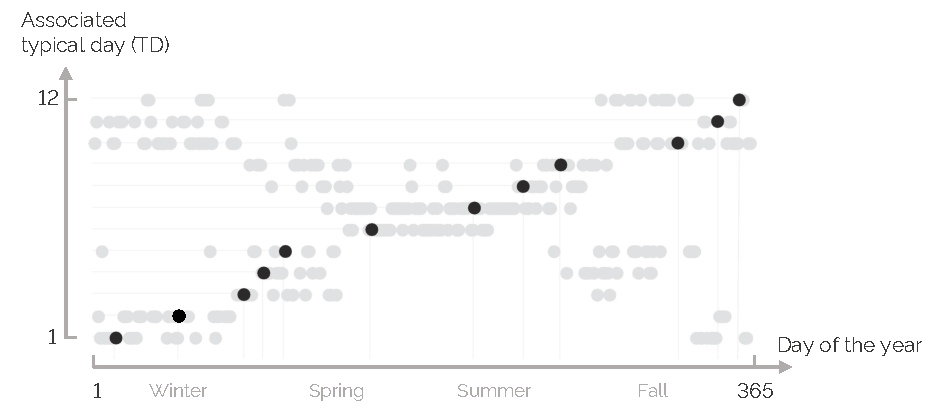
\includegraphics[width=0.9\textwidth]{Typical_days.pdf}
\caption{Association of each day of the year (gray dots) to one of the 12 typical days (TDs) (black dots). Graph adapted from \citet{limpens2019energyscope}.}
\label{fig:Typical_days}
\end{figure}

Finally, to properly capture the inter days dynamics, EnergyScope TD uses the ``Coupling typical days'' method from \citet{Gabrielli2018}. Among others, this allows representing the dynamics and the seasonality of storage capacities. This method as well as the clustering approach selected in our case, \ie k-medoids \cite{Kaufman2009,Park2009}, are extensively detailed and compared to other methods, in the work of \citet{limpens2019energyscope}. \\

\myparagraph{Overview of the snapshot model}\\

\noindent
EnergyScope TD \cite{limpens2019energyscope} is a model that optimises both the investment and operating strategy of a '\emph{whole}'-energy system, encompassing electricity, heating, mobility, and non-energy sectors. According to \citet{contino2020whole}, a model qualifies as a 'whole-energy' system when it considers all energy sectors, including the non-energy demand such as the production of plastics and other materials using feedstocks that are also considered as energy carriers, with the same level of detail.

The model's hourly resolution over a year makes it well-suited for integrating intermittent renewables. Its formulation incorporates a reconstruction method that captures different time scales from the hour to the season while accounting for the inter-weeks patterns of wind. The model optimises the investment decisions and hourly operations over a year, with a computational time of less than a minute on a personal laptop. This characteristic was intentionally incorporated into the model design to facilitate uncertainty quantification and other studies that require numerous iterations \cite{rixhon2021role}.

EnergyScope TD has been successfully applied to various national energy systems, including Switzerland \cite{Limpens_role_2019,limpens2019energyscope}, Belgium \cite{Limpens2020}, Italy \cite{borasio2022deep}, and other European countries \cite{dommisse2020modelling}. Furthermore, it has been extended to a multi-region energy system model \cite{thiran2023validation}, coupled with other energy models \cite{pavivcevic2022bidirectionnal}, or employed to focus on specific sectors such as the networks of electricity, gas, and hydrogen \cite{schnidrig2023role}.\\

\myparagraph{Formulation of the snapshot model}\\

\noindent
The conceptual structure of the model is illustrated in Figure \ref{fig:estd_overview}: given the end-use energy demand, the efficiency and cost of energy conversion technologies, the availability and cost of energy resources, the model identifies the optimal investment and hourly operation strategies to meet the demand and minimise the total annual cost and greenhouse gas emissions of the energy system. Typically, the two objectives are integrated by placing a limit on emissions while simultaneously minimizing the costs. 

 \begin{figure}[!htbp]
\centering
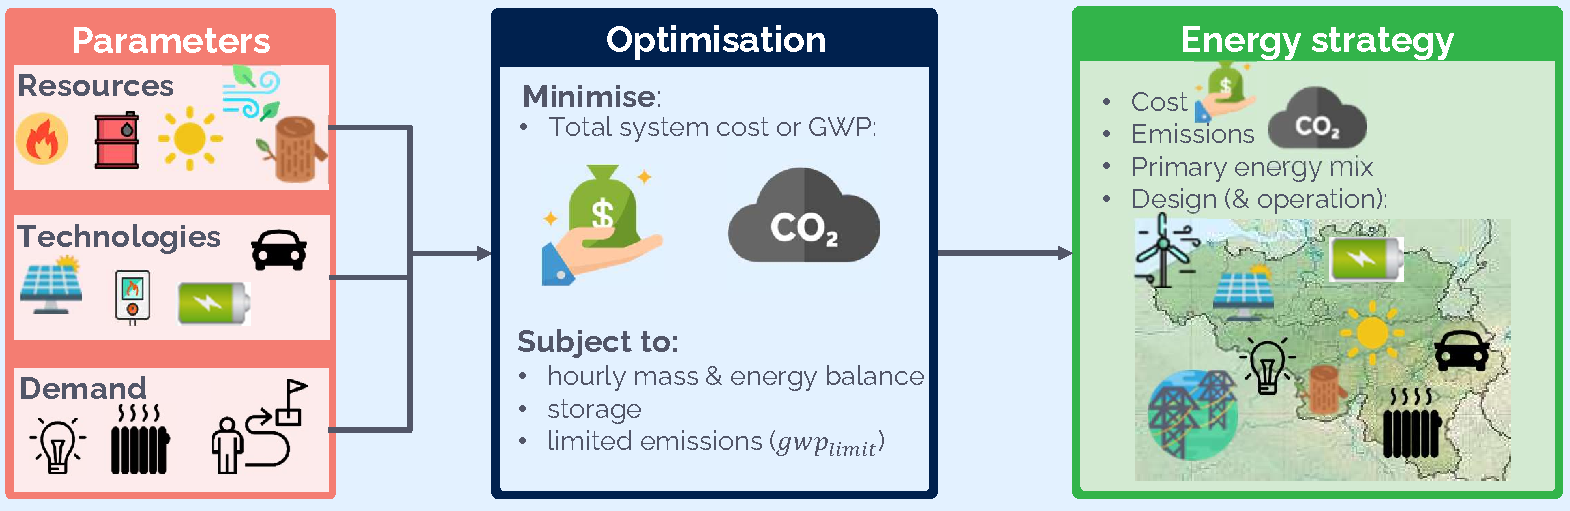
\includegraphics[width=\textwidth]{chp_estd_overview.pdf}
\caption{EnergyScope TD model is a flow model with inputs (Parameters), an optimizing model (Optimisation) and results (Energy strategy). }
\label{fig:estd_overview}
\end{figure}


\myparagraph{Linear formulation}\\

\noindent
The following section illustrates the formulation of the original EnergyScope TD model. The objective function, cost and \gls{GHG} formulation are detailed. The rest of the formulation is detailed and available in a previous work \cite{limpens2021generating}. 
This work uses the following nomenclature: SETs are in capital letters, \textbf{Variables} are in bold and with the first letter in upper case, and \emph{parameters} are in italic. 

\begingroup
\belowdisplayskip=2pt
\abovedisplayskip=2pt
\begin{flalign} 
% Objective function + investment 
\label{eq:obj_func_app}%1
% adding 25pt space, otherwise flalign with two "&" would flush to the extreme left
\hspace{0pt} \min \text{  } & \textbf{C\textsubscript{tot}} = \sum_{\mathclap{j \in \text{\emph{TECH}}}} \Big(\textbf{$\tau$}(j) \textbf{C\textsubscript{inv}}(j) + \textbf{C\textsubscript{maint}} (j)\Big) + \sum_{\mathclap{i \in \text{\emph{RES}}}} \textbf{C\textsubscript{op}}(i)&\\
\label{eq:tau_app}%2
 \text{s.t. } & \textbf{$\tau$}(j) =  \frac{i_{\text{\emph{rate}}}(i_{\text{\emph{rate}}}+1)^{\emph{lifetime}(j)}}{\left(\left(i_{\text{\emph{rate}}}+1\right)^{\emph{lifetime}(j)}\right) - 1} & \forall j \in \text{\emph{TECH}}
% \label{eq:c_inv_app}%3
% & \textbf{C\textsubscript{inv}}(j) = c_{\text{\emph{inv}}}(j) \textbf{F}(j) & \forall j \in \text{\emph{TECH}}\\
% \label{eq:c_maint_app}%4
% & \textbf{C\textsubscript{maint}}(j) = c_{\text{\emph{maint}}}(j) \textbf{F}(j) & \forall j \in \text{\emph{TECH}}\\ 
%  \label{eq:c_op_app}%5
% & \textbf{C\textsubscript{op}}(i) = \sum_{\mathclap{t \in T }} c_{\text{\emph{op}}}(i) \textbf{F\textsubscript{t}}(i,t) t_{op} (t)  
% & \forall i \in \text{\emph{RES}}
 \end{flalign}
 \endgroup
 
The objective, Equation (\ref{eq:obj_func_app}), is the minimisation of the total annual cost of the energy system (\textbf{C\textsubscript{tot}}), defined as the sum of the annualised investment cost of the technologies (\textbf{$\tau$}$\cdot$\textbf{C\textsubscript{inv}}), the operating and maintenance costs of the technologies (\textbf{C\textsubscript{maint}}) and the operating cost of the resources (\textbf{C\textsubscript{op}}).
The annualised factor $\tau$ is computed \emph{a priori} based on the interest rate (\emph{i\textsubscript{rate}}) and the technology lifetime, (\emph{lifetime}), Equation (\ref{eq:tau_app}).


\begingroup
\belowdisplayskip=2pt
\abovedisplayskip=2pt
\begin{flalign} 
% Objective function + investment 
%\label{eq:obj_func_app}%1
%% adding 25pt space, otherwise flalign with two "&" would flush to the extreme left
%\hspace{0pt} \min \text{  } & \textbf{C\textsubscript{tot}} = \sum_{\mathclap{j \in \text{\emph{TECH}}}} \Big(\textbf{$\tau$}(j) \textbf{C\textsubscript{inv}}(j) + \textbf{C\textsubscript{maint}} (j)\Big) + \sum_{\mathclap{i \in \text{\emph{RES}}}} \textbf{C\textsubscript{op}}(i)&\\
%\label{eq:tau_app}%2
% \text{s.t. } & \textbf{$\tau$}(j) =  \frac{i_{\text{\emph{rate}}}(i_{\text{\emph{rate}}}+1)^{\emph{lifetime}(j)}}{\left(\left(i_{\text{\emph{rate}}}+1\right)^{\emph{lifetime}(j)}\right) - 1} & \forall j \in \text{\emph{TECH}}\\
 \label{eq:c_inv_app}%3
 & \textbf{C\textsubscript{inv}}(j) = c_{\text{\emph{inv}}}(j) \textbf{F}(j) & \forall j \in \text{\emph{TECH}}\\
 \label{eq:c_maint_app}%4
 & \textbf{C\textsubscript{maint}}(j) = c_{\text{\emph{maint}}}(j) \textbf{F}(j) & \forall j \in \text{\emph{TECH}}
%  \label{eq:c_op_app}%5
% & \textbf{C\textsubscript{op}}(i) = \sum_{\mathclap{t \in T }} c_{\text{\emph{op}}}(i) \textbf{F\textsubscript{t}}(i,t) t_{op} (t)  
% & \forall i \in \text{\emph{RES}}
 \end{flalign}
 \endgroup

The total investment cost (\textbf{C\textsubscript{inv}}) of each technology results from the multiplication of its specific investment cost (\emph{c\textsubscript{inv}}) and its installed capacity (\textbf{F}), see Equation (\ref{eq:c_inv_app}).  The installed capacity is defined with respect to the main end-uses output type, such as electricity for \gls{PV} or heat for a boiler. The total operation and maintenance costs (\textbf{C\textsubscript{maint}}) are calculated in the same way, Equation (\ref{eq:c_maint_app}). 


\begingroup
\belowdisplayskip=2pt
\abovedisplayskip=2pt
\begin{flalign} 
% Objective function + investment 
%\label{eq:obj_func_app}%1
%% adding 25pt space, otherwise flalign with two "&" would flush to the extreme left
%\hspace{0pt} \min \text{  } & \textbf{C\textsubscript{tot}} = \sum_{\mathclap{j \in \text{\emph{TECH}}}} \Big(\textbf{$\tau$}(j) \textbf{C\textsubscript{inv}}(j) + \textbf{C\textsubscript{maint}} (j)\Big) + \sum_{\mathclap{i \in \text{\emph{RES}}}} \textbf{C\textsubscript{op}}(i)&\\
%\label{eq:tau_app}%2
% \text{s.t. } & \textbf{$\tau$}(j) =  \frac{i_{\text{\emph{rate}}}(i_{\text{\emph{rate}}}+1)^{\emph{lifetime}(j)}}{\left(\left(i_{\text{\emph{rate}}}+1\right)^{\emph{lifetime}(j)}\right) - 1} & \forall j \in \text{\emph{TECH}}\\
% \label{eq:c_inv_app}%3
% & \textbf{C\textsubscript{inv}}(j) = c_{\text{\emph{inv}}}(j) \textbf{F}(j) & \forall j \in \text{\emph{TECH}}\\
% \label{eq:c_maint_app}%4
% & \textbf{C\textsubscript{maint}}(j) = c_{\text{\emph{maint}}}(j) \textbf{F}(j) & \forall j \in \text{\emph{TECH}}\\ 
  \label{eq:c_op_app}%5
 & \textbf{C\textsubscript{op}}(i) = \sum_{\mathclap{t \in T }} c_{\text{\emph{op}}}(i) \textbf{F\textsubscript{t}}(i,t) t_{op} (t)  
 & \forall i \in \text{\emph{RES}}
 \end{flalign}
 \endgroup



The total cost of the resources (\textbf{C\textsubscript{op}}) is calculated as the sum of the end-use over the different time-periods multiplied by the period duration (\emph{t\textsubscript{op}}) and the specific cost of the resources (\emph{c\textsubscript{op}}), Equation (\ref{eq:c_op_app}). To simplify the reading, we write the sum over typical days as $t\in T$ such as in Equation (\ref{eq:c_op_app}). The period $T$ represents the sequence of hours and typical days over a year (8760h)\footnote{The exception is storage level which is optimised over the 365 days of the year instead of typical days.}. The full formulation is detailed in \cite{limpens2019energyscope} or in the documentation \cite{readthedocs_estd_v2.2}.

\begingroup
\belowdisplayskip=2pt
\abovedisplayskip=2pt
\begin{flalign}
 \label{eq:GWP_tot_app}%8
 \phantom{\hspace{0pt} \min \text{  } }
 & \textbf{GWP\textsubscript{tot}}  =    \sum_{\mathclap{i \in \text{\emph{RES}}}} \textbf{GWP\textsubscript{op}} (i) 
 &\\
  \label{eq:GWP_op_app}%7
 & \textbf{GWP\textsubscript{op}}(i) = \sum_{\mathclap{t \in T }} \emph{gwp}_{\text{\emph{op}}}(i) \textbf{F\textsubscript{t}}(i,t)  t_{op} (t) & \forall i \in \text{\emph{RES}}
\end{flalign}
\endgroup

 
The global annual \gls{GHG} emissions are calculated using a \gls{LCA} approach, i.e. taking into account emissions of the resources `\emph{from cradle to use}'. It is based on the indicator `\emph{GWP100a-IPCC2013}´ developed by the \acrfull{IPCC} \cite{IPCC2014}. For climate change, the natural choice as indicator is the \acrlong{GWP}, expressed in ktCO$_2$-eq./year. In Equation (\ref{eq:GWP_tot_app}), the total yearly emissions  of the system (\textbf{GWP\textsubscript{tot}}) are defined as the emissions related to resources (\textbf{GWP\textsubscript{op}}). The total emissions of the resources are the emissions associated to fuels (from cradle to combustion) and imports of electricity (\emph{gwp\textsubscript{op}}) multiplied by the period duration  (\emph{t\textsubscript{op}}), Equation (\ref{eq:GWP_op_app}).
Thus, this version accounts only for operation without accounting for the \gls{GWP} emitted during the construction of the technologies. This makes the results comparable with metrics used in the reports by the European Commission and the \acrfull{IEA}.


The above equations (Equations (\ref{eq:obj_func_app}) - (\ref{eq:GWP_op_app})) represent only a part of the formulation and illustrate the syntax that is used. Those representing the energy balance, network implementation, sectors representation, etc. are not presented in this work but are detailed in the latest version of the model, see \cite{limpens2021generating} and in the documentation \cite{readthedocs_estd_v2.2}. 

Finally, energy storage has two dimensions to be optimised: (i) the hourly power flow, encompassing both charging and discharging and, (ii) the stored energy quantity (also referred to as 'storage level'). EnergyScope TD optimises the former based on the hourly resolution of the typical days and the latter over the entire span of 8760 hours in a year. This formulation allows for the effective integration of a wide range of energy storage technologies, spanning short-term solutions like small thermal storage units and daily-use batteries, to longer-term options such as hydro-dam storage for seasonal storage, and even large-scale thermal storage for intra-week patterns. A previous study investigated the roles of various storage technologies, considering their sectoral applications and temporal aspects, within the context of the Swiss energy system \cite{Limpens_role_2019}.

\subsection{Extending the model for pathway optimisation}
\label{sec:path_methodo}

In this section, we delve into the extension of EnergyScope TD from a static yearly snapshot model to a comprehensive pathway model. While snapshot models provide insights into the energy system for individual years, they lack the capacity to capture the dynamics inherent in investment strategies throughout a transition period. The proposed approach involves segmenting the transition into five-year intervals. This approach results in seven instances of EnergyScope TD -- called representative years -- spanning the 30-year transition period, covering the years from 2020 to 2050. To bridge these representative years, we introduce additional constraints that capture the investments changes between consecutive periods, accounting for societal inertia and evaluating both the cost implications and emissions of the transition (see Figure \ref{fig:meth_path_methodology}). Overall, these constraints are integrated into a linear framework, ensuring computational efficiency, with an approximate computational time of 14 minutes on a personal laptop (2.4 GHz Intel Core i5 quad-core). Simplification and choices were necessary to implement linearly the problem while keeping a tractable computational time. In this section, the retained formulation is presented.

\begin{figure}[!htbp]
\centering
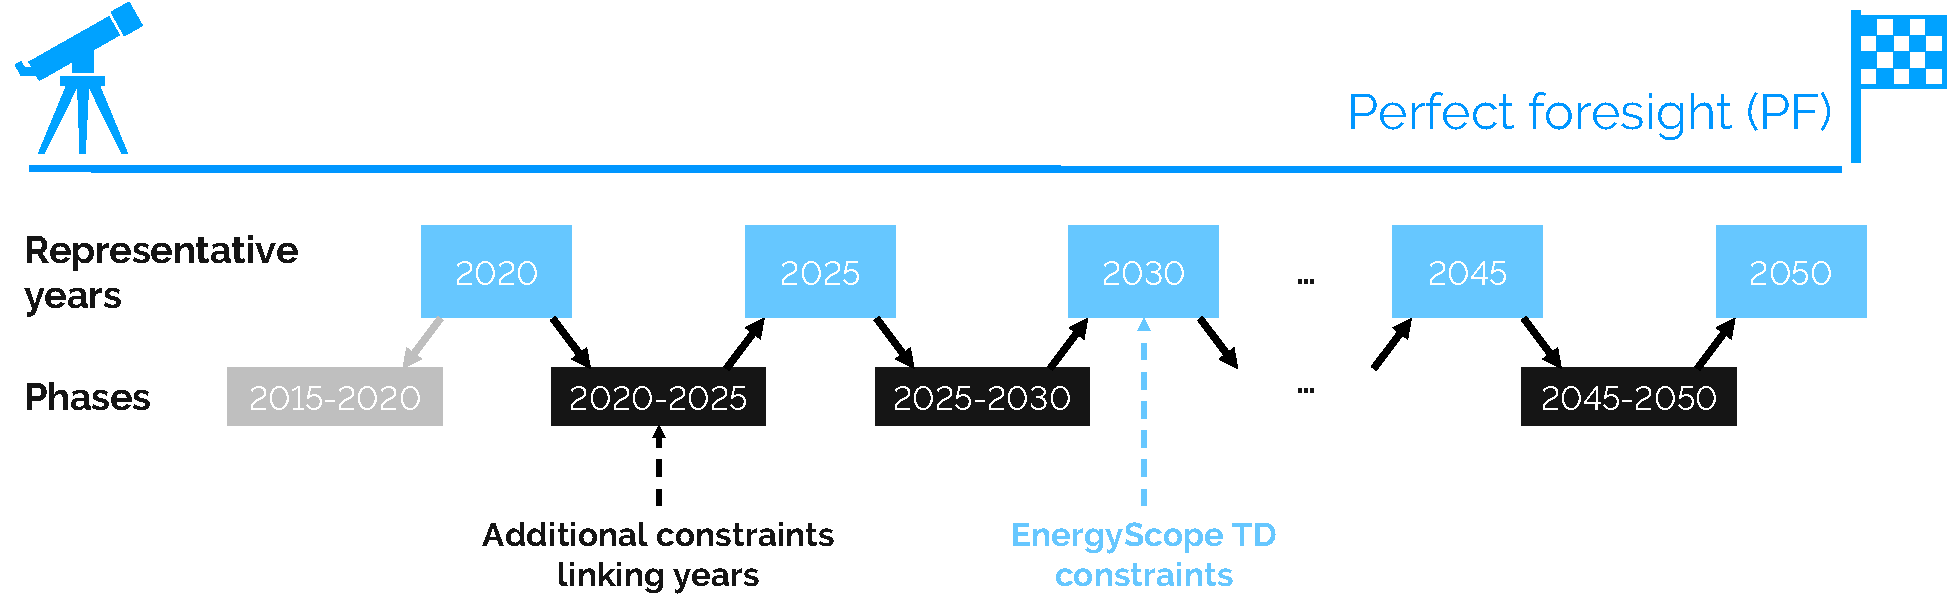
\includegraphics[width=\textwidth]{ES_Pathway.pdf}
\caption{The pathway methodology relies on 7 representative years (blue boxes) where the model \gls{ESTD} is applied. Moreover, the formulation accounts for linking constraints (black boxes) and an initial condition (grey box). The overall problem is the pathway model.}
\label{fig:meth_path_methodology}
\end{figure}

The proposed formulation relies on representative years, selected every 5 years from 2020 to 2050.  The period between two of them is called `\emph{PHASE}´.
For each of these 7 representative years, the EnergyScope TD model is run  using the relevant data (such as energy demand, technology costs or \gls{GHG} emissions constraints). 

As a consequence, a new dimension `\emph{year}' is added to all \textbf{Variables} and parameters, except the interest rate (\emph{i\textsubscript{rate}}) assumed constant during the transition. This new dimension is necessary to represent the changes of technology and resource characteristics over the representative years. 
As an example, the investment cost (\emph{c}\textsubscript{\emph{inv}}) of solar photovoltaic panels could drastically vary in the next decades (e.g. data used ranges between 1220 to 870  [€/kW] between 2020 and 2035). \\

\myparagraph{Linking years}\\

\noindent
At this stage, all years are independent. In the following, we introduce new constraints to link representative years. The formulation allows to install new capacity (\textbf{F\textsubscript{new}}), remove a capacity that has reached  its lifespan (\textbf{F\textsubscript{old}}) or decommission a technology prematurely (\textbf{F\textsubscript{decom}}). These capacity changes occur during a phase, this implies that there is no capacity change during a representative year. Figure \ref{fig:path_eg_igcc} illustrates the concept.

\begin{figure}[!htbp]
\centering
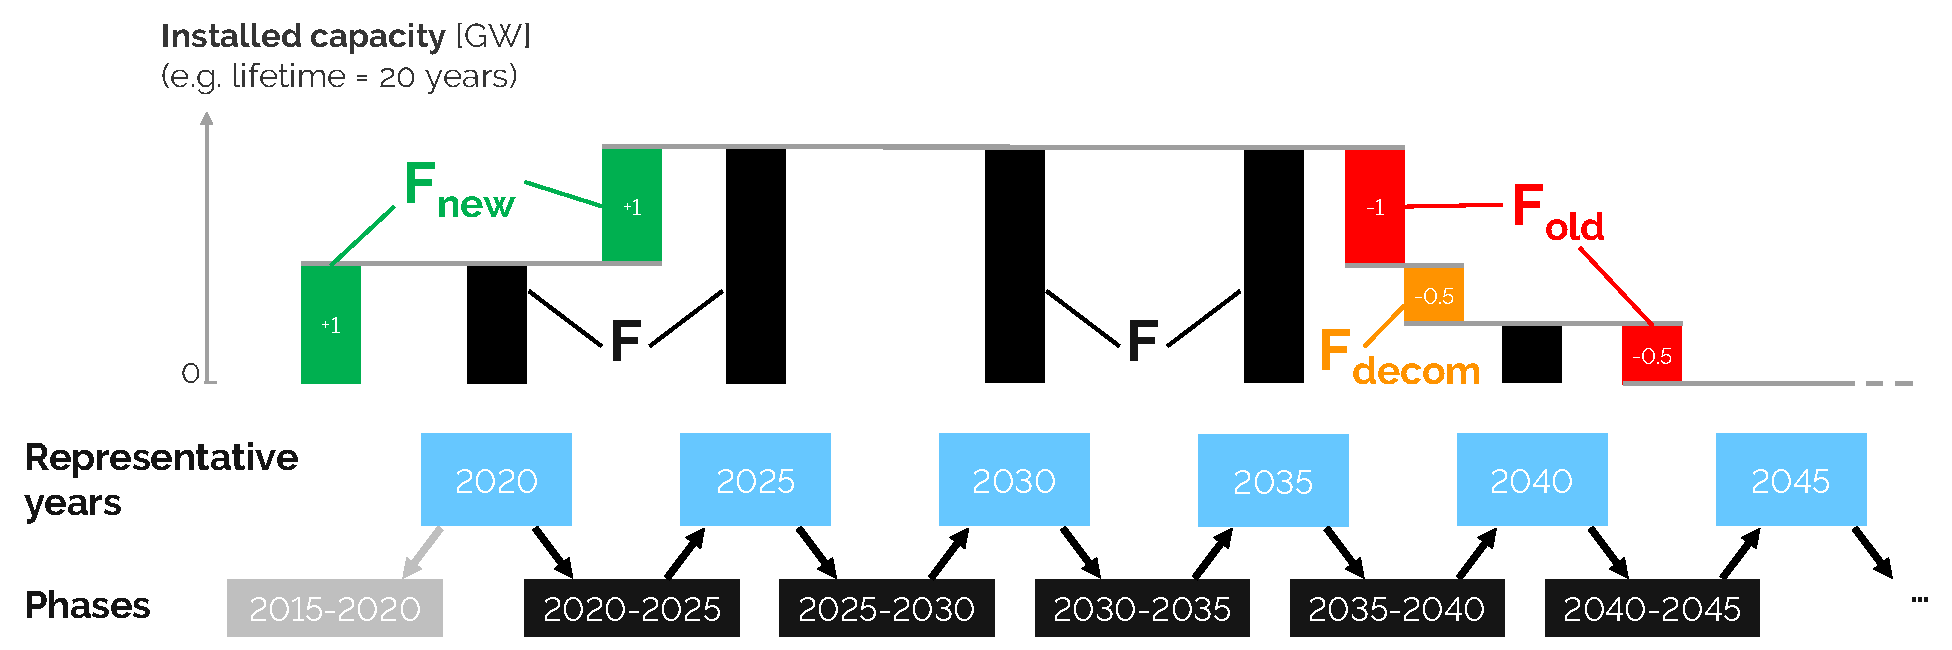
\includegraphics[width=\textwidth]{path_e.g._tech.pdf}
\caption{Example of how the technology capacities and associated variables are evolving. The example uses a technology with a 20 years lifetime. Initially 1~GW of capacity exists (\textbf{F\textsubscript{new}} during phase $2015\_2020$). Then another 1~GW is deployed (\textbf{F\textsubscript{new}} during phase $2020\_2025$). 15 years later, a part of the capacity reaches its lifetime limit and is removed (\textbf{F\textsubscript{old}} phase $2035\_2040$). 
Moreover, during the latter phase, additional capacity is decommissioned  prematurely (\textbf{F\textsubscript{decom}}). Finally, the technology reaches its expected lifetime and is fully withdrawn (\textbf{F\textsubscript{old}}).}
\label{fig:path_eg_igcc}
\end{figure}

\begingroup
\belowdisplayskip=2pt
\abovedisplayskip=2pt
\begin{flalign} 
\label{eq:F_newBuilt_app}%5
&\textbf{F}(y\textsubscript{stop},i) = \textbf{F}(y\textsubscript{start},i)
 + \textbf{F\textsubscript{new}}(p,i)
 - \textbf{F\textsubscript{old}}(p,i)
 - \sum_{\mathclap{p2 \in \text{\emph{PHASE}} \cup \{2015\_2020\}}} \textbf{F\textsubscript{decom}}(p,p2,i)& \notag \nonumber 
 \end{flalign}
\begin{flalign} 
 &&  \forall p \in \text{\emph{PHASE}}, \emph{y\textsubscript{stop}} \in \emph{Y\_STOP}(p), \emph{y\textsubscript{start}} \in \emph{Y\_START}(p), i \in \text{\emph{TECH}}
 \end{flalign}

\endgroup
 
Similarly to a mass balance, Equation (\ref{eq:F_newBuilt_app}) is the technology capacity balance. The constraint forces the installation or withdrawing of capacities between two representative years: 
at the end of the phase (\emph{y\textsubscript{stop}}), the available capacity is the one used in the next representative year (\textbf{F}(\emph{y\textsubscript{stop}})). This capacity is equal to the one available in the previous representative year (\textbf{F}(\emph{y\textsubscript{start}})) plus the new installed capacity (\textbf{F\textsubscript{new}}) minus the capacity that has reached its lifetime (\textbf{F\textsubscript{old}}) minus the early decommissioned capacity (\textbf{F\textsubscript{decom}}). One notices that the capacity available for each representative year depends on a year (\emph{y\textsubscript{start}} or \emph{y\textsubscript{stop}}), while the other capacity changes depend on a phase (\emph{p} or \emph{p}2). Moreover, the decommissioning term depends on another phase, which is the one when the technology decommissioned has been built. As an illustration, Figure \ref{fig:path_eg_igcc} gives an example where 0.5 GW of a capacity built in 2015\_2020 is decommissioned in 2030\_2035 (\textbf{F\textsubscript{decom}}(2030\_2035,2015\_2020,i)). 

 \begingroup
\belowdisplayskip=2pt
\abovedisplayskip=2pt
\begin{flalign} 
 & \textbf{F\textsubscript{decom}}(p,p2,i) = 0 \hspace{-2cm}&
\notag \nonumber
 \end{flalign}
\begin{flalign} 
  \label{eq:F_decomNonPhysic1_app}
& &  \forall i \in \emph{TECH}, p\in \emph{PHASE}, p2 \in \emph{PHASE} \cup \{2015\_2020\} | \emph{decom\textsubscript{allowed}}(p,p2) = 0 & 
 \end{flalign}
  \begin{flalign}
 \label{eq:Fold_def_app}%1
&\textbf{F\textsubscript{old}} (p,i) =  
\hspace{3mm}\text{if} ( \emph{age} = \text{`\emph{STILL\_IN\_USE}'}) \text{ then} 0   &   &\notag\nonumber\\
&\hspace{2cm}\text{else } \left(\textbf{F\textsubscript{new}}(age,i)  - \sum_{\vspace{5mm}\mathclap{p2 \in \text{\emph{PHASE}}}} \textbf{F\textsubscript{decom}} (p2,age,i)\right)    & \notag\nonumber\\
&& \hspace{-5cm} \forall p \in PHASE , \forall j \in TECH | age \in AGE(p,j)
 \end{flalign}
\endgroup

In linear programming, a solution might be mathematically correct, while not making sense in practice. As an example, a technology could be decommissioned before being built ($ \emph{p} < \emph{p\textsubscript{built}}$). Equations (\ref{eq:F_decomNonPhysic1_app}-\ref{eq:Fold_def_app})  allow preventing these non-sense while keeping the formulation linear. 
Equation (\ref{eq:F_decomNonPhysic1_app}) forces the decommissioned capacity to zero when technology will be built after.
To do so, a parameter (\emph{decom\textsubscript{allowed}}) is defined \emph{a priori} and is equal to 0 or 1 when decommissioning is not possible or possible, respectively. 
Equation (\ref{eq:Fold_def_app}) defines the capacity reaching its lifetime limit at a certain phase, the concept is illustrated in Figure \ref{fig:path_eg_igcc}. For each phase, a set (\emph{AGE}) is calculated \emph{a priori}. It relates, for a given phase and technology, when the technology was built.  
In the case the technology has already reached its lifetime limit, the set (\emph{AGE}) returns the phase when the technology has been built. The first part of Equation (\ref{eq:Fold_def_app}) indicates that the technology is still available, and thus no capacity needs to be removed. The second part of the equation represents the capacity that reached its expected lifetime minus a part of the capacity that would have been decommissioned. 
As an example, Figure \ref{fig:path_eg_igcc} shows a 20 years lifetime technology with 1~GW of capacity installed before 2020. 
The `if' in Equation (\ref{eq:Fold_def_app}) is linear as it is applied to a parameter and not a variable. 

 \begingroup
\belowdisplayskip=2pt
\abovedisplayskip=2pt
\begin{flalign} 
 \label{eq:Phase2020Design_app}
& \textbf{F\textsubscript{new}}(\emph{2015\_2020},i) = \textbf{F}(\emph{YEAR\_2020},i)& \forall i \in \emph{TECH}
 \end{flalign}
\endgroup

To initialise the problem in 2020 with the existing design, an additional phase `\emph{2015\_2020}' is created. Equation (\ref{eq:Phase2020Design_app}) requires that the capacity used in 2020 is installed in the previous phase. \\

\myparagraph{Society inertia}\\

\noindent
To avoid unrealistically fast changes in the system, additional constraints are needed during the phases for the mobility and low temperature heat sectors. Without the following constraints, the model would eliminate certain technologies in one phase, such as oil and gas decentralised boilers. Even if this result is mathematically and physically correct, (\ie fuels are expensive and investing in more efficient technology is economically and environmentally more profitable), this swap of technology cannot occur in one phase (\ie 5 years). Indeed, society inertia to change, available manpower, supply chains and manufacturers limit the change.

\begingroup
\belowdisplayskip=2pt
\abovedisplayskip=2pt
\begin{flalign} 
\label{eq:delta_tech_during_phase_app}
& \textbf{$\Delta$\textsubscript{change}}(p,i) \geq 
   \sum_{\mathclap{t \in T }} \left( \textbf{F\textsubscript{t}}(\emph{y\textsubscript{start}},i,t) \right) 
   -\sum_{\mathclap{t \in T }} \left( \textbf{F\textsubscript{t}}(\emph{y\textsubscript{stop}},i,t) \right)&\notag\nonumber\\
&&\hspace{-8cm} \forall j \in \emph{TECH}, p \in \emph{PHASE}, \emph{y\textsubscript{start}} \in \emph{Y\_START}(p), \emph{y\textsubscript{stop}} \in \emph{Y\_STOP}(p)
 \end{flalign}
 \begin{flalign}
\label{eq:limit_reno_LTheat_app}
&\sum_{\mathclap{\hspace{2cm}i\in TECH(HeatLowT)}} \textbf{$\Delta$\textsubscript{change}}(p,i) 
\leq
 \emph{lim\textsubscript{LT,ren}} \cdot 
\big( {eui}(\emph{y\textsubscript{start}},HotWater)  +  \emph{eui}(\emph{y\textsubscript{start}},SpaceHeat)  \big)\hspace{-1cm}&\notag\nonumber\\
&\hspace{5.5cm} \forall p \in \emph{PHASE}, \emph{y\textsubscript{start}} \in \emph{Y\_START}(p) & \\
\label{eq:limit_reno_passmob_app}
&\sum_{\mathclap{\hspace{2cm}i\in TECH(MobPass)}} \textbf{$\Delta$\textsubscript{change}}(p,i) 
\leq
 \emph{lim\textsubscript{MobPass}} \cdot \emph{eui}(\emph{y\textsubscript{start}},MobPass) )&\notag\nonumber\\
&\hspace{5.5cm} \forall p \in \emph{PHASE}, \emph{y\textsubscript{start}} \in \emph{Y\_START}(p) & \\
\label{eq:limit_reno_freight_app}
&\sum_{\mathclap{\hspace{2cm}i\in TECH(MobFreight)}} \textbf{$\Delta$\textsubscript{change}}(p,i) 
\leq
 \emph{lim\textsubscript{MobFreight}} \cdot \emph{eui}(\emph{y\textsubscript{start}},MobFreight) &\notag\nonumber\\
&\hspace{5.5cm} \forall p \in \emph{PHASE}, \emph{y\textsubscript{start}} \in \emph{Y\_START}(p) &
\end{flalign}
\endgroup

%\hspace{3cm} euc \in EUT\_OF\_CAT(HeatLowT),i\in \emph{TECH\_OF\_EUT}(euc)
%\hspace{3cm} euc \in EUT\_OF\_CAT(MobPass),i\in \emph{TECH\_OF\_EUT}(euc)
%\hspace{3cm} euc \in EUT\_OF\_CAT(MobFreight),i\in \emph{TECH\_OF\_EUT}(euc)

Equation (\ref{eq:delta_tech_during_phase_app}) calculates the upper limit of change (\textbf{$\Delta$\textsubscript{change}}) in terms of supplied demand instead of installed capacity. 
%% GL_correction_v2 %% Following line added:
%  Ici on prend la différence entre ystart et ystop (et non pas le contraire), en effet, on est intéressé par la réticence des personnes à se séparer de leur ancienne technologie, plutot que la réticense à accepter une nouvelle techno. 
%% GL_correction_v2 %% end
Based on this quantification, the amount of change per phase is limited for low temperature heat (\emph{lim\textsubscript{LT,ren}}), Equation (\ref{eq:limit_reno_LTheat_app}), passenger mobility (\emph{lim\textsubscript{MobPass}}), Equation (\ref{eq:limit_reno_passmob_app}) and freight mobility (\emph{lim\textsubscript{MobFreight}}), Equation (\ref{eq:limit_reno_freight_app}). 
For instance, if the maximum allowable variation in supplied low temperature heat is set at 25\%, it would restrict the technology-related changes in low temperature heat to 25\% within a given phase. Consequently, if a technology supplies more than 25\% of the low temperature heat, it would require multiple phases to replace it with a different technology.\\
%As an example, setting the maximum change of supplied heat at low temperature to 25\% would limit the change in technology related to heat at low temperature to 25\% during a phase. 
%In this case, if more than 25\% of the low temperature heat was supplied by a technology, it would take more than one phase to replace it by a different one.


\myparagraph{Cost and emissions of the transition}\\

\noindent
To optimise the energy system, two key metrics must be adapted: the transition cost and the total \acrfull{GWP}. 
Concerning the first one, all costs are expressed in €\textsubscript{2020} and an annualisation factor is used to distinguish investments over the transition. For the \gls{GWP}, the metric used is based on the contributions of the gases over 100 years. It is assumed that the impact of emitting at the beginning or the end of transition are equivalent and thus no annualisation is used. 


\begingroup
\belowdisplayskip=2pt
\abovedisplayskip=2pt
\begin{flalign} 
% Objective function + investment 
\label{eq:obj_func_v2_app}%1
% adding 25pt space, otherwise flalign with two "&" would flush to the extreme 
\hspace{0pt} \min \text{  } & \textbf{C\textsubscript{tot,trans}} = \textbf{C\textsubscript{tot,capex}} + \textbf{C\textsubscript{tot,opex}}&\\
\label{eq:Capex_v2_app}
& \textbf{C\textsubscript{tot,capex}} =
\sum_{\mathclap{p \in \text{\emph{PHASE}}\cup \{2015\_2020\}}} 
\textbf{C\textsubscript{inv,phase}}(p)
-
\sum_{\mathclap{i \in \emph{TECH}}} 
\textbf{C\textsubscript{inv,return}}(i)\\
  \label{eq:Copex_tot_v2_app}%5
& \textbf{C\textsubscript{tot,opex}} =  \textbf{C\textsubscript{opex}}(2020)
+ \emph{t\textsubscript{phase}}\cdot \tau\textsubscript{\emph{phase}}(p) \cdot \sum_{\mathclap{p \in \emph{PHASE}|y\textsubscript{start}\in \emph{P\_START}(p),y\textsubscript{stop}\in \emph{P\_STOP}(p)}} 
 \Big(\textbf{C\textsubscript{opex}}(y\textsubscript{start}) + \textbf{C\textsubscript{opex}}(y\textsubscript{stop}) \Big)/2&\\
\label{eq:path_annu_factor_app}
& \tau\textsubscript{\emph{phase}}(p) = 1/(1+\emph{i\textsubscript{rate}})^{\emph{diff\_2015\_year(p)}} &
%% GL_correction_v2 %% & \tau\textsubscript{\emph{phase}}(p) = 1/(1+\emph{i\textsubscript{rate}})^{\emph{diff\_2015\_year(p)}} &
\end{flalign}
\endgroup

As an extension of Equation \ref{eq:obj_func_app}, the objective function to be minimised is the total transition cost of the energy system (\textbf{C\textsubscript{tot,trans}}), 
defined as the sum of the total \gls{CAPEX} (\textbf{C\textsubscript{tot,capex}}) and the \gls{OPEX} (\textbf{C\textsubscript{tot,opex}}), according to Equation (\ref{eq:obj_func_v2_app}). The total \gls{CAPEX} (\textbf{C\textsubscript{tot,capex}}) is the sum of the investment during each phase (\textbf{C\textsubscript{inv,phase}}), Equation (\ref{eq:Capex_v2_app}), to which the residual asset value in 2050 is withdrawn (\textbf{C\textsubscript{inv,return}}). Thus, the investments account for the installation and dismantlement costs of the technologies. The total \gls{OPEX} (\textbf{C\textsubscript{tot,opex}}) is the sum of the \gls{OPEX} in 2020 and the annualised sum of the \gls{OPEX} during each phase (\textbf{C\textsubscript{opex}}), Equation (\ref{eq:Copex_tot_v2_app}). During a phase, the system \gls{OPEX} is 
the product of the annualised phase factor, defined in Equation (\ref{eq:path_annu_factor_app}), and the arithmetic average of \gls{OPEX} cost for the representative years before and after the phase. The annualised phase factor is defined based on an average interest rate during the transition.
%assumed to be the annualised average of its first and last year. The annualised phase factor  ($\tau$\textsubscript{\emph{phase}}) is defined in Eq.~(\ref{eq:path_annu_factor_app}).

\begingroup
\belowdisplayskip=2pt
\abovedisplayskip=2pt
\begin{flalign} 
\label{eq:opex_yearly_app}
&\textbf{C\textsubscript{opex}} (y) = \sum_{\mathclap{i \in \emph{TECH}}} \textbf{C\textsubscript{maint}}(y,i) + \sum_{\mathclap{j \in \emph{RES}}} \textbf{C\textsubscript{op}}(y,j)&\forall y\in \emph{YEARS}
\end{flalign}
\endgroup

For each year, the yearly \gls{OPEX} (\textbf{C\textsubscript{opex}}) is the sum of the operating and maintenance costs of technologies (\textbf{C\textsubscript{maint}}) and  the operating cost of the resources (\textbf{C\textsubscript{op}}), Equation (\ref{eq:opex_yearly_app}).

\begingroup
\belowdisplayskip=2pt
\abovedisplayskip=2pt
\begin{flalign} 
\label{eq:PhaseInv_app}%5
&\textbf{C\textsubscript{inv,phase}}(p) = \sum_{\mathclap{j \in \emph{TECH}}} \textbf{F\textsubscript{new}}(p,j)\cdot \tau\textsubscript{\emph{phase}}(p)\cdot \left(\emph{c\textsubscript{inv}}(\emph{y\textsubscript{start}},j) + \emph{c\textsubscript{inv}}(\emph{y\textsubscript{stop}},j)\right)/2&\notag\nonumber
\end{flalign}
\begin{flalign}
&&\forall p \in \emph{PHASE} | y\textsubscript{start}\in \emph{P\_START}(p),y\textsubscript{stop}\in \emph{P\_STOP}(p)
\end{flalign}
\endgroup

The investment during a phase (\textbf{C\textsubscript{inv,phase}}) results from the multiplication of the newly built technologies (\textbf{F\textsubscript{new}}) with their annualised arithmetic averaged specific cost, Equation (\ref{eq:PhaseInv_app}). The annualised phase factor  (defined by Equation (\ref{eq:path_annu_factor_app})) is used. The specific cost during the phase is defined as  the average between the investment cost for the first and last year of the period. 


\begingroup
\belowdisplayskip=2pt
\abovedisplayskip=2pt
\begin{flalign} 
\label{eq:salvage_app}%5
&\textbf{C\textsubscript{inv,return}}(i) = \hspace{2.5cm}
\sum_{\mathclap{p \in \emph{PHASE}\cup \{2015\_2020\}|y\textsubscript{start}\in \emph{Y\_START}(p),y\textsubscript{stop}\in \emph{Y\_STOP}(p)}} 
\hspace{0.5cm}
 \tau_{phase}(p)\cdot \left(c_{inv}(y_{start},i)+c_{inv}(y_{stop},i)\right)/2 \cdot
&\notag\nonumber
\end{flalign}
\begin{flalign}
& 
\hspace{1.7cm}
\frac{remaining\_years(i,p)}{\emph{lifetime}(y\textsubscript{start},i)} \left( \textbf{F\textsubscript{new}}(p,i) - 
\sum_{\mathclap{p2 \in \emph{PHASE}}} 
\textbf{F\textsubscript{decom}}(p2,p,i)\right)&
\forall i \in \emph{TECH}
\end{flalign}
\endgroup

A part of the investment will remain after 2050. This residual investment, also called salvage value, can be calculated for each technology. 
A parameter, calculated \textit{a priori} , gives for each technology and construction phase, the remaining amount of years (\emph{remaining\_years}). 
As an example, if a PV panel has been built in 2045 and has a 20 years lifetime, the parameter will equal to 15 years. 
Thus, the salvage value is a fraction of the investment cost of this technology when it has been built. 
This fraction is the ratio between the number of remaining years and the lifetime of the technology. 
In the previous example, the residual investment of the PV built is 75\%. 
Equation (\ref{eq:salvage_app}) computes, for each technology, the residual value that must be subtracted from the total cost. The residual value reflects the fact that the technology can still be used after the horizon of the model and is not fully amortised. The residual value is not applied to technologies that are removed prematurely. This differ from other models, such as Plexos where a technology removed prematurely will benefit from its salvage value (see analysis of \cite{waucquez2023validation}).

\begingroup
\belowdisplayskip=2pt
\abovedisplayskip=2pt
\begin{flalign} 
\label{eq:gwp_tot_transition_app}
&\textbf{GWP\textsubscript{tot,trans}}= \textbf{GWP\textsubscript{tot}}(2020) + \emph{t\textsubscript{phase}}\sum_{\mathclap{p \in \emph{PHASE}|y\textsubscript{start}\in \emph{Y\_START}(p),y\textsubscript{stop}\in \emph{Y\_STOP}(p)}}/2 \left(\textbf{GWP\textsubscript{tot}}(y\textsubscript{start}) +\textbf{GWP\textsubscript{tot}}(y\textsubscript{stop}) \right)&
\\
\label{eq:limit_gwp_trans_app}
& \textbf{GWP\textsubscript{tot,trans}} \leq \emph{gwp\textsubscript{lim,trans}}&
\end{flalign}
\endgroup

The total \acrfull{GWP} emissions during the transition (\textbf{GWP\textsubscript{tot,trans}}) are equal to the sum of the total emissions per period (\textbf{GWP\textsubscript{tot}}), Equation (\ref{eq:gwp_tot_transition_app}). The emissions during a phase is estimated as the arithmetic average of the representative years before and after the phase. Equation (\ref{eq:limit_gwp_trans_app}) limits the total \gls{GWP} emissions during the transition by a maximum (\emph{gwp\textsubscript{lim,trans}}).